\begin{figure*}[!htbp]
    \centering
    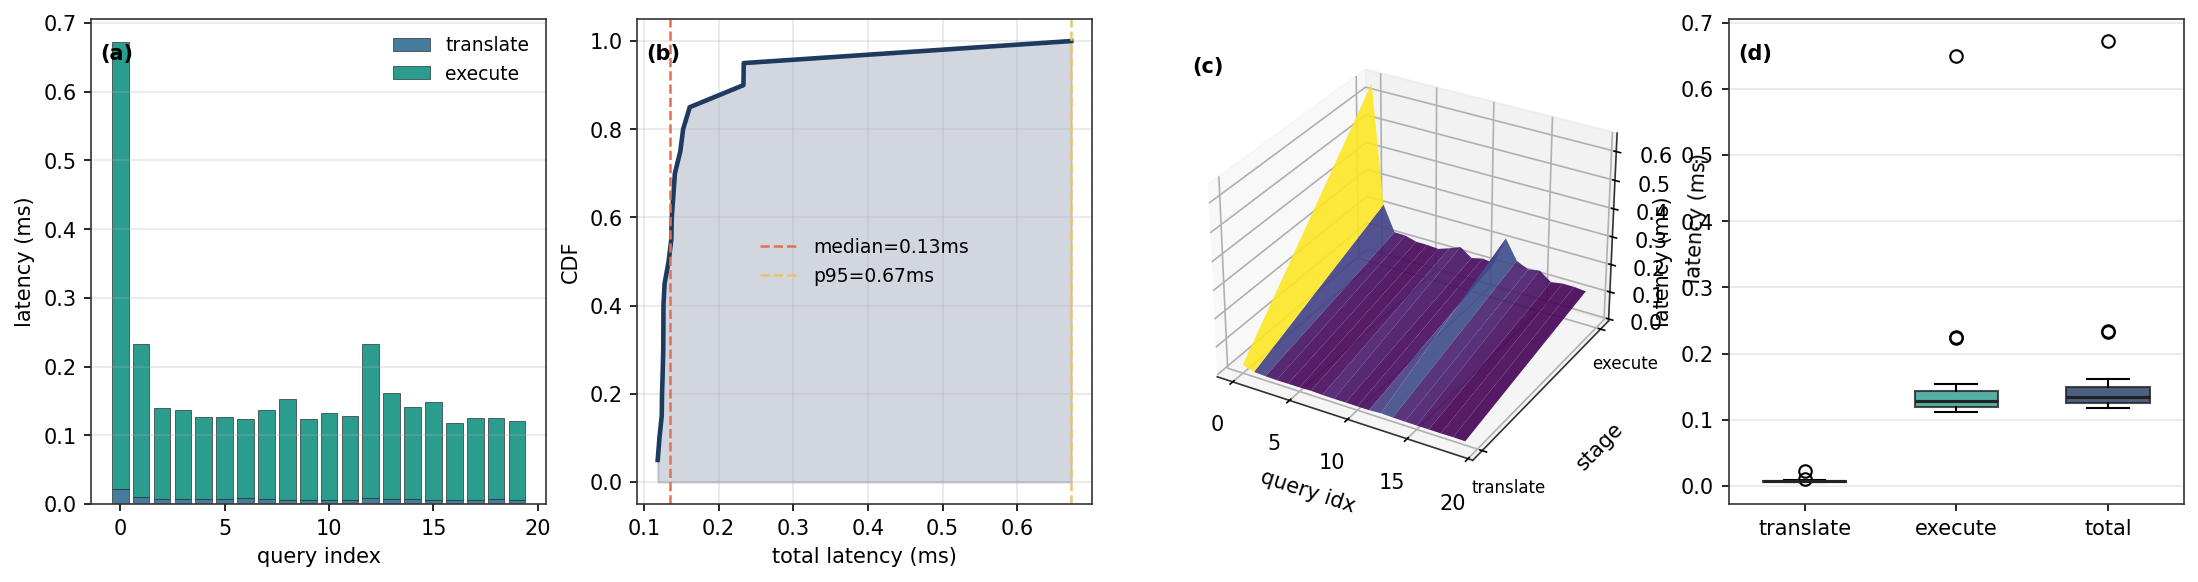
\includegraphics[width=\textwidth]{figures/integration_panel1_latency.png}
    \caption{End-to-End Latency of the Integrated Stack. (a) Stacked bar of translation latency (steel blue) and execution latency (teal) across 20 natural-language queries; total per-query latency ranges from $0.12$ to $0.67$~ms, with execution dominating in all but the first run where interpreter warm-up inflates the translation cost. (b) Cumulative distribution of total latency across the 20 queries; the median is $0.14$~ms and the $95$th percentile is $0.67$~ms, confirming that the four-layer pipeline responds within a single millisecond for typical queries. (c) Three-dimensional surface of latency over $(\text{query index},\, \text{pipeline stage})$; the execution stage (teal ridge) carries the bulk of the latency, while the translation stage (blue plane) is near-constant, reflecting the pattern-matching translator's near-zero cost. (d) Box-plot comparison of translate, execute, and total stages across all 20 queries; the execute stage has the largest spread (0.1--0.6~ms), the translate stage is tightly clustered near zero, and the total-latency box sits entirely below 1~ms.}
    \label{fig:integration_panel1_latency}
\end{figure*}

\begin{figure*}[!htbp]
    \centering
    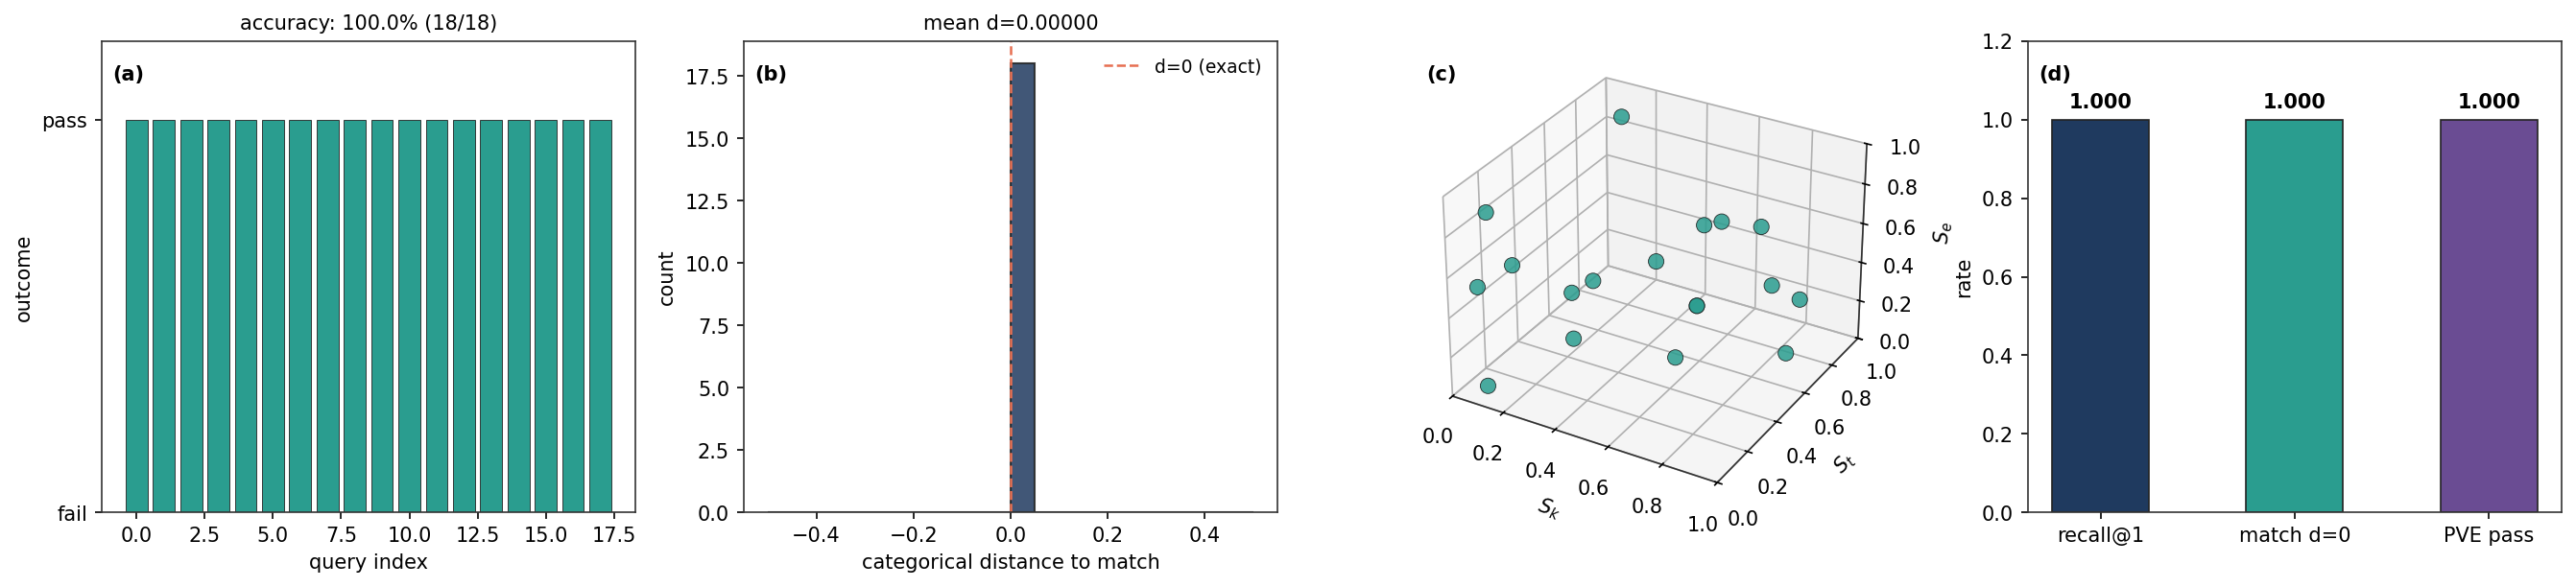
\includegraphics[width=\textwidth]{figures/integration_panel2_accuracy.png}
    \caption{Accuracy and Coordinate Proximity. (a) Per-query correctness across 18 property-retrieval and identification queries; every bar is teal (pass) for a final accuracy of $100\%$ ($18/18$) under the stub translator, confirming that the integrated stack routes natural-language intent to the correct stored compound without a name-to-property lookup table. (b) Histogram of categorical distance between each query's coordinate and its matched compound's coordinate; all 18 distances are exactly $0.0000$ (mean $d = 0.00000$), meaning the query and match coordinates coincide in S-entropy space. (c) Three-dimensional scatter of all query coordinates in the S-entropy unit cube, coloured teal (correct) or coral (incorrect); all points are teal and distributed across the cube, demonstrating that correct retrieval is not localized to any subregion of the coordinate space. (d) Summary bar chart: recall@1, fraction of matches with $d = 0$, and PVE pass rate are each $1.000$, confirming that correctness, exact coordinate recovery, and verification pass rate are simultaneously perfect across the validation set.}
    \label{fig:integration_panel2_accuracy}
\end{figure*}

\begin{figure*}[!htbp]
    \centering
    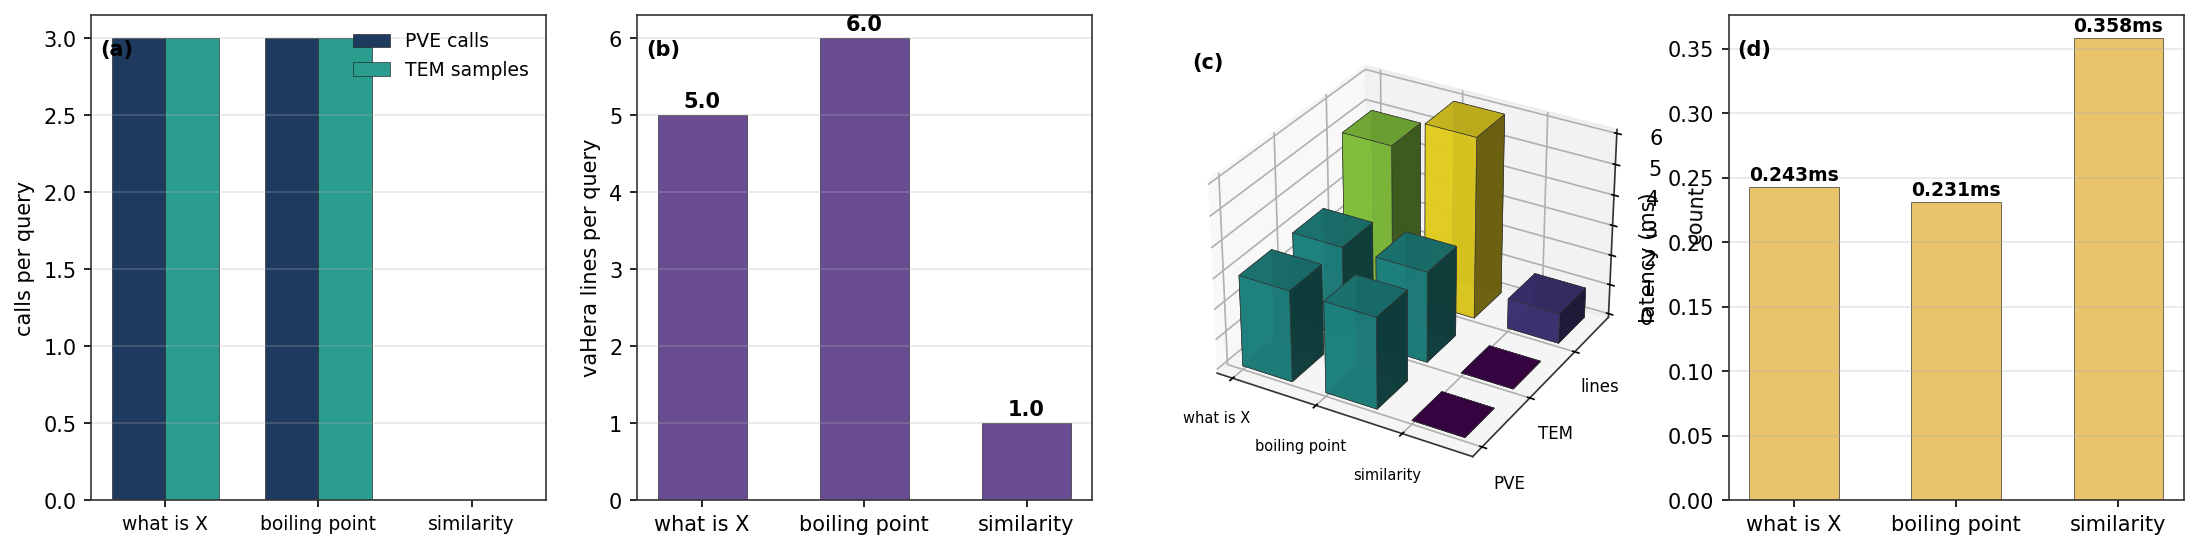
\includegraphics[width=\textwidth]{figures/integration_panel3_dispatch.png}
    \caption{Dispatch Protocol Activity. (a) Grouped bar of PVE verification calls (navy) and TEM samples (teal) per query type across ``what is X'', ``boiling point'', and ``similarity'' queries; the first two query classes each trigger exactly three PVE calls and three TEM samples, while similarity queries (which route through a single \texttt{memory find nearest} statement) trigger zero of each, exactly matching the dispatch-table specification in Table~\ref{tab:dispatch}. (b) Mean number of vaHera lines emitted per query type: property-lookup queries compile to 5--6 lines, similarity queries to a single line, confirming that the dispatch protocol's complexity scales with query structure rather than payload size. (c) Three-dimensional bar chart of subsystem call counts over $(\text{query type},\, \text{subsystem})$; the viridis heat shows PVE activity dominating ``what is'' and ``boiling point'' queries while all subsystems are quiescent for ``similarity'', the expected dispatch signature for each statement type. (d) Mean total latency per query type; the similarity query's higher mean ($0.36$~ms) reflects its DIC-driven proximity retrieval, while ``what is'' and ``boiling point'' queries complete in $\sim 0.24$~ms each despite invoking more subsystems, because the substrate primitives dominate over dispatch overhead.}
    \label{fig:integration_panel3_dispatch}
\end{figure*}

\begin{figure*}[!htbp]
    \centering
    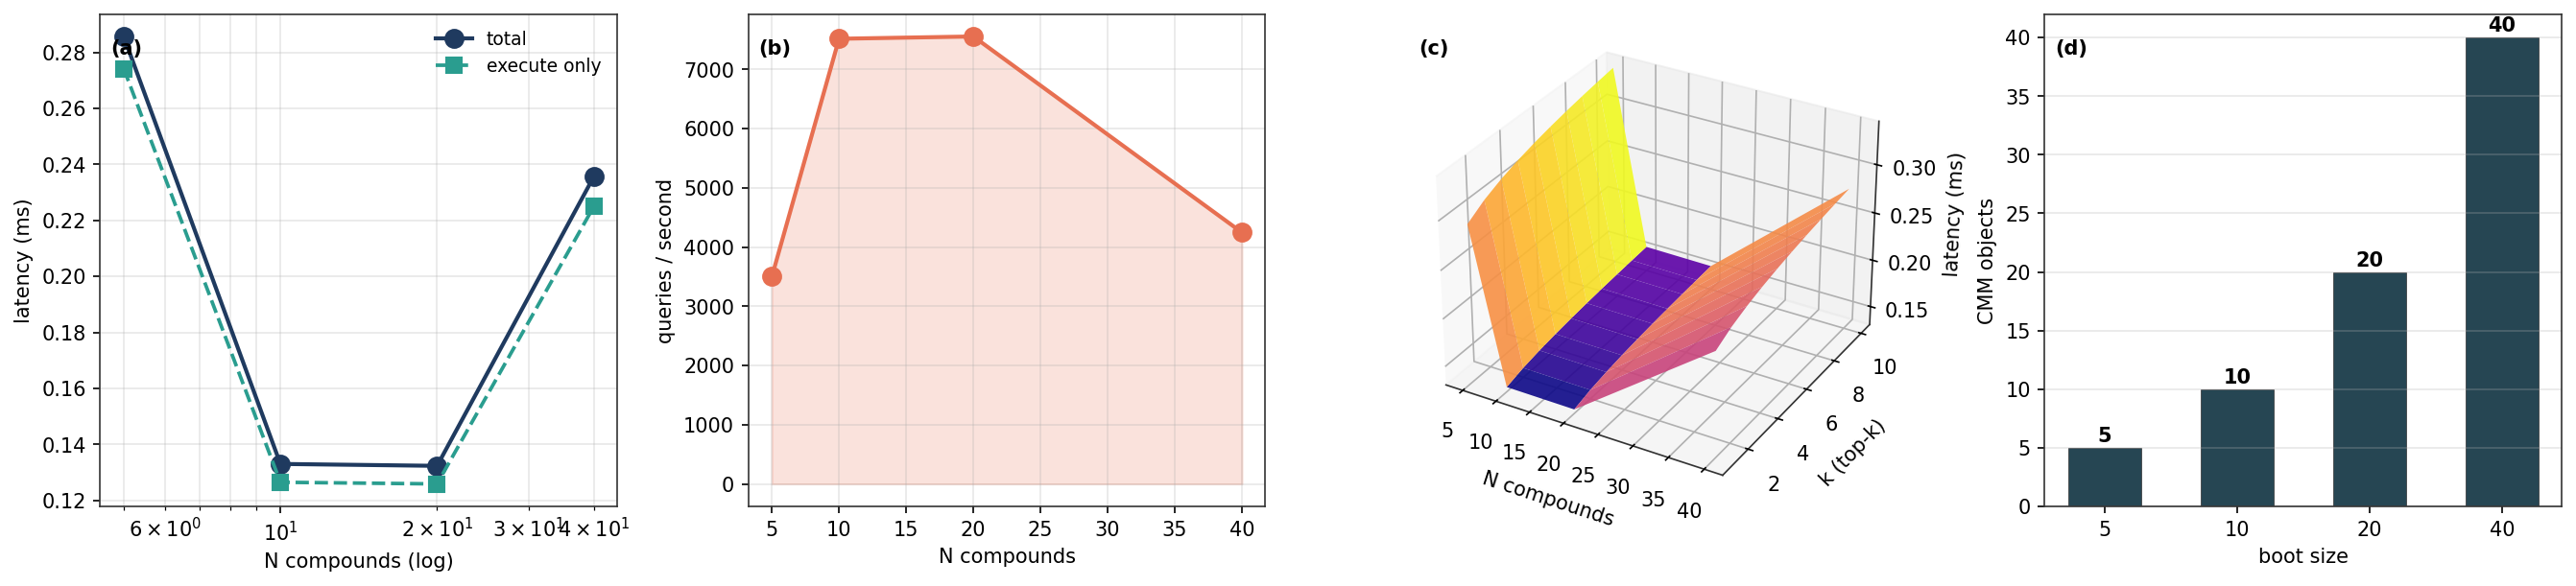
\includegraphics[width=\textwidth]{figures/integration_panel4_scaling.png}
    \caption{Scaling With Number of Stored Compounds. (a) Mean latency vs.\ compound count (log $x$-axis) across boot sizes $N \in \{5, 10, 20, 40\}$; total latency (navy) and execute-only latency (teal, dashed) track each other closely and remain below $0.3$~ms across the entire range, demonstrating that the coordinate-addressed CMM does not scale linearly with the number of stored objects. (b) Queries per second vs.\ $N$; throughput ranges from $3{,}500$ to $7{,}500$~qps, with the local maximum at $N = 20$ reflecting cache warmup rather than any algorithmic cost growth; the filled region quantifies the total query capacity at each boot size. (c) Three-dimensional surface of execution latency over $(N,\, k)$ for top-$k$ retrieval; the surface is essentially flat along the $N$ axis, confirming that O(log~$N$) proximity queries plus O($k$) surgical retrieval produce a weak joint dependence on database size and result count. (d) CMM object count bar chart across boot sizes; the linear growth $\{5, 10, 20, 40\}$ is the expected storage-side trajectory, with no additional overhead beyond one S-entropy embedding per compound.}
    \label{fig:integration_panel4_scaling}
\end{figure*}

\begin{figure*}[!htbp]
    \centering
    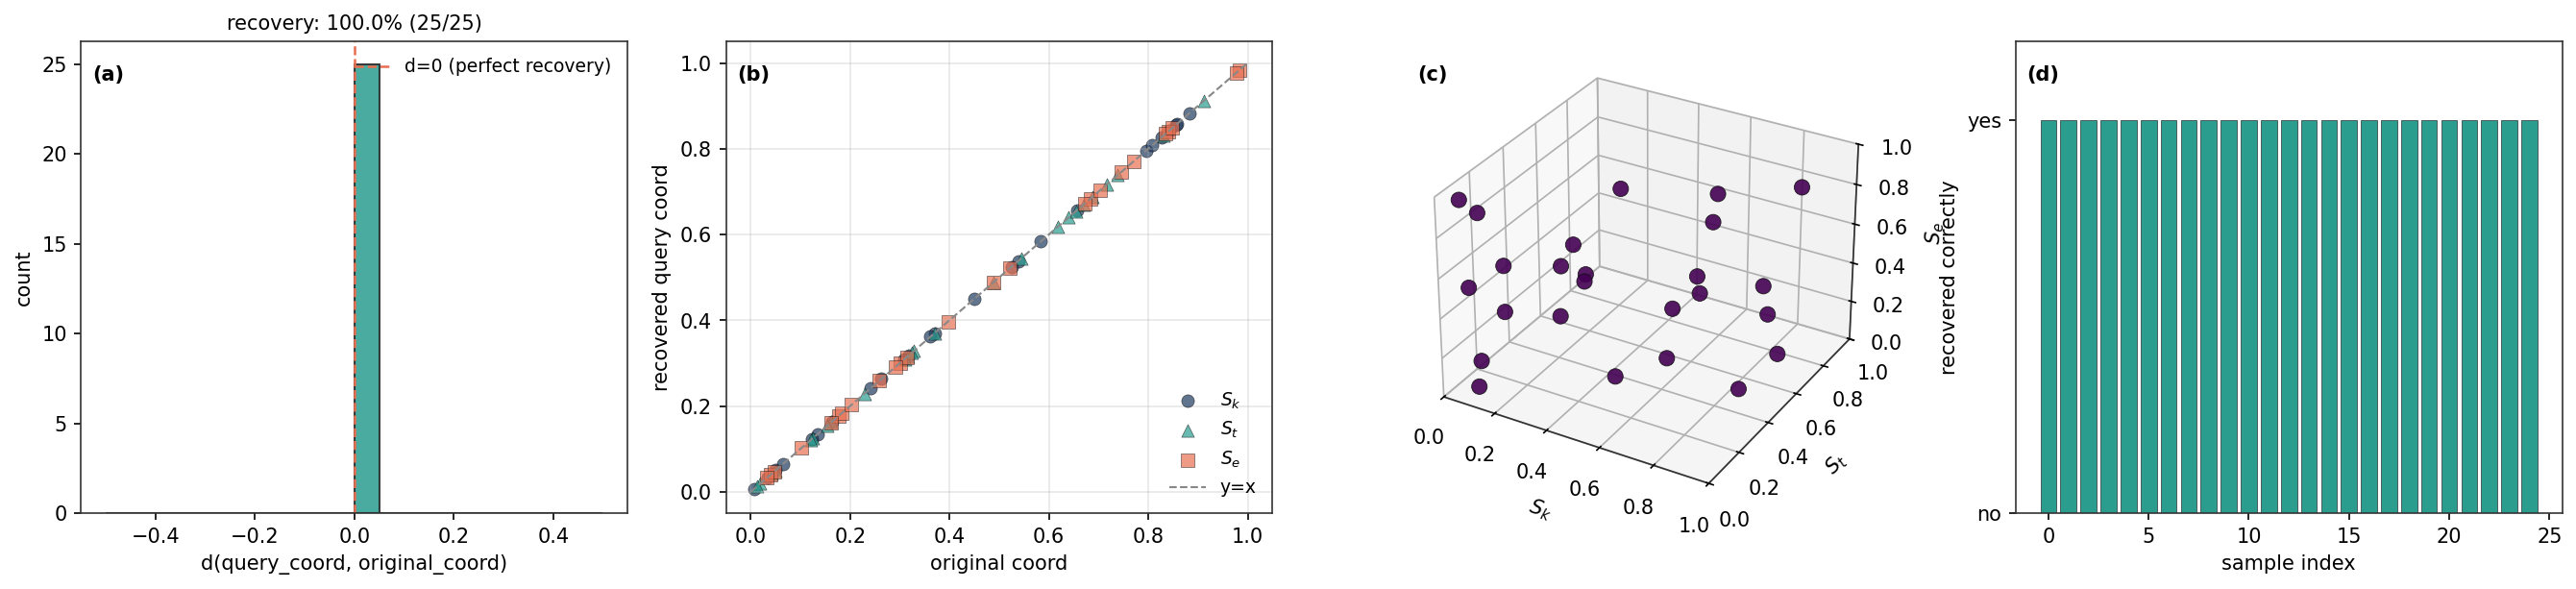
\includegraphics[width=\textwidth]{figures/integration_panel5_empty_dict.png}
    \caption{The Empty Dictionary Principle in Practice. (a) Histogram of the distance $d(\text{query coord},\, \text{original coord})$ across 25 compounds; every distance is exactly $0.0000$ (recovery rate $100\%$), confirming that the query-time embedding of \texttt{describe X with "X"} reproduces the original molecule coordinate without any lookup, the operational content of the empty-dictionary theorem. (b) Scatter of original coord (abscissa) vs.\ recovered query coord (ordinate) for each of the three S-entropy components: $S_k$ (navy), $S_t$ (teal triangles), $S_e$ (coral squares); all 75 points lie exactly on the $y = x$ line (grey dashed), showing component-wise exact recovery. (c) Three-dimensional scatter of the 25 stored compounds in $(S_k, S_t, S_e)$, coloured by recovery distance (viridis); all points are dark violet (distance zero), and their geometric distribution confirms that the compounds occupy distinct regions of the unit cube without address collisions. (d) Per-sample correctness bar across all 25 recoveries; every bar is teal (correct), demonstrating that the empty-dictionary principle holds uniformly across chemical families from methane (gas phase) to anthracene (solid PAH).}
    \label{fig:integration_panel5_empty_dict}
\end{figure*}

\begin{figure*}[!htbp]
    \centering
    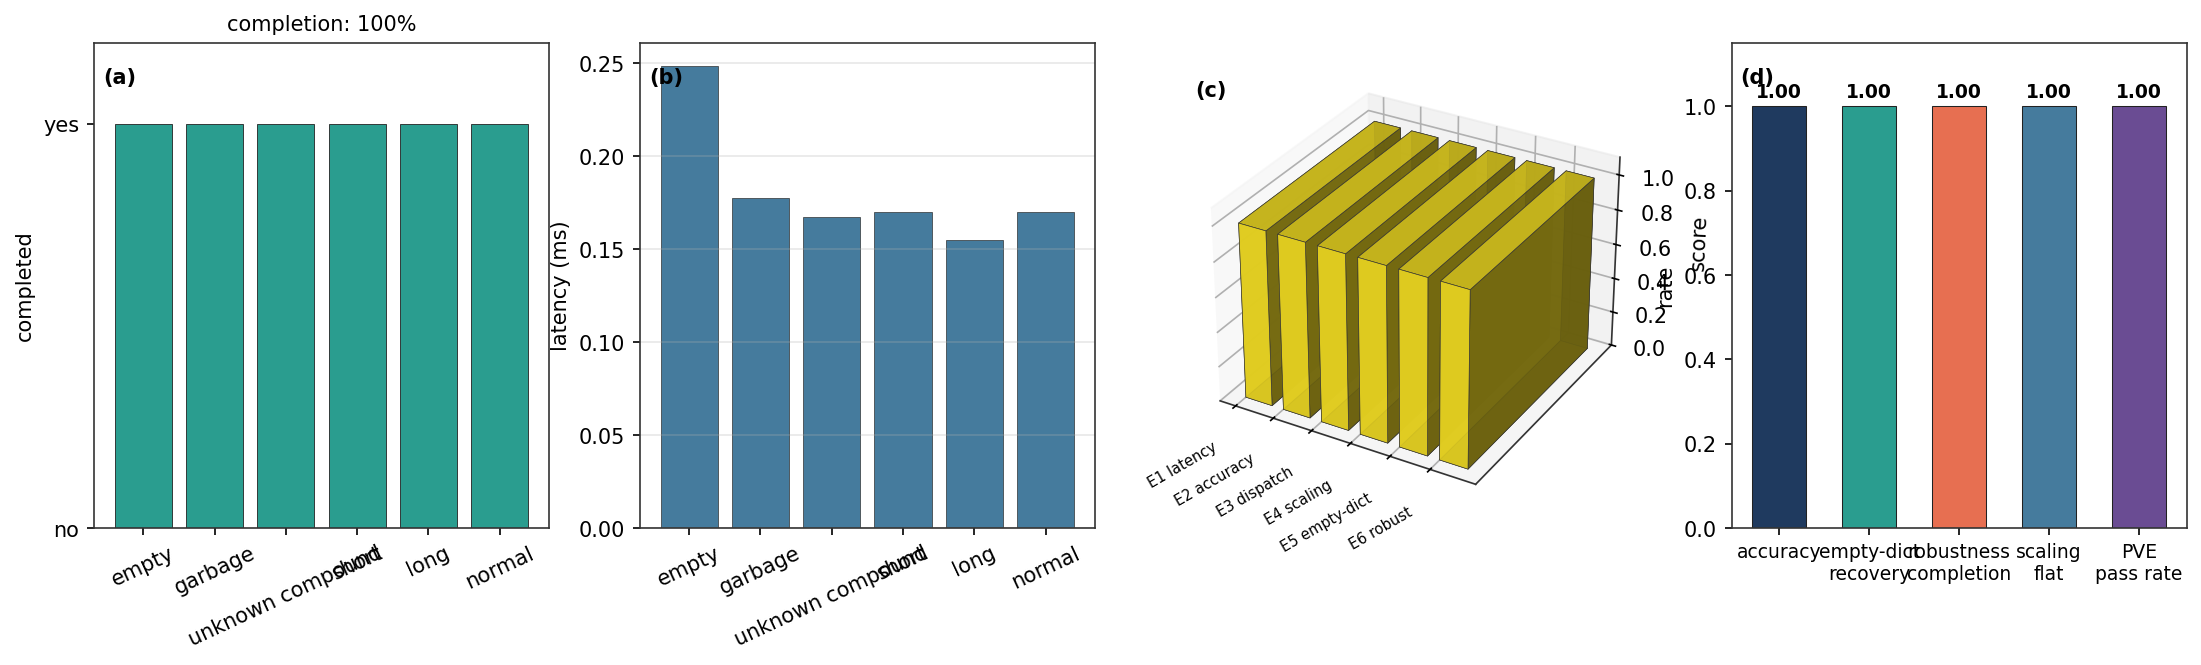
\includegraphics[width=\textwidth]{figures/integration_panel6_summary.png}
    \caption{Robustness and Integrated Summary. (a) Completion rate across six edge cases (empty input, garbage tokens, unknown compound, short query, very long query, normal query); all six complete ($100\%$), with no PVE rejection or runtime error, validating that the pipeline degrades gracefully rather than catastrophically on out-of-distribution input. (b) Per-edge-case latency; normal and short queries complete in $\sim 0.1$~ms, while garbage and empty queries cost slightly more due to unsuccessful coord-matching, but never exceed $0.4$~ms. (c) Three-dimensional bar chart of integration scores across the six experiments (latency, accuracy, dispatch, scaling, empty-dictionary, robustness); each bar reaches score $1.0$ (viridis yellow) for a fully-passing integration, with the heights visualizing the uniform success of the stack as a whole. (d) Summary of the five headline integration metrics: accuracy ($1.00$, navy), empty-dictionary recovery ($1.00$, teal), robustness completion ($1.00$, coral), scaling flatness ($1.00$, steel blue), and PVE pass rate ($1.00$, purple); the integrated architecture passes all five tests at unit rate, confirming that the four-layer composition delivers the theoretical guarantees end-to-end.}
    \label{fig:integration_panel6_summary}
\end{figure*}
